% Final paper -- Artificial Intelligence and Economic Modeling (UP 2026-II)
%
% Body: 8 to 20 pages in THIS format (11pt, 1-inch margins, single column).
% Do not change the geometry or the font size to fit the limit.
% References and appendices do not count towards the limit.
\documentclass[11pt]{article}
\usepackage[utf8]{inputenc}
\usepackage[T1]{fontenc}
\IfFileExists{spanish.ldf}{\usepackage[spanish,es-nodecimaldot,es-noshorthands,es-lcroman]{babel}}{}
\usepackage[margin=1in]{geometry}
\usepackage{amsmath,amssymb,amsthm}
\usepackage{bbm}
\usepackage{booktabs}
\usepackage{graphicx}
\usepackage{xcolor}
\usepackage[round]{natbib}
\usepackage[colorlinks=true,allcolors=blue!50!black]{hyperref}

\newtheorem{proposition}{Proposición}
\newtheorem{lemma}{Lema}
\newtheorem{corollary}{Corolario}
\theoremstyle{definition}
\newtheorem{assumption}{Supuesto}
\newtheorem{definition}{Definición}
\newtheorem{remark}{Observación}

\newcommand{\E}{\mathbb{E}}
\newcommand{\1}{\mathbbm{1}}
\IfFileExists{../code/output/numbers.tex}{\newcommand{\tauShareMin}{18}
\newcommand{\tauShareMax}{22}
\newcommand{\tauMin}{0.05}
\newcommand{\tauMax}{0.09}
\newcommand{\DeltaDataMin}{0.25}
\newcommand{\DeltaDataMax}{0.46}
\newcommand{\habitDecayMax}{0.009}
\newcommand{\objMzero}{1{,}451}
\newcommand{\objMone}{1{,}430}
\newcommand{\objBest}{1{,}276}
\newcommand{\bestModel}{M2}
\newcommand{\betaStatic}{2.22}
\newcommand{\betaBest}{1.37}
\newcommand{\lamBest}{0.37}
\newcommand{\rhoBest}{0.95}
\newcommand{\peakBest}{43}
\newcommand{\nMoments}{222}
}{}

\title{La brecha de participación a los 70 años sobrestima el efecto del voto obligatorio:\\
\large ciclo de vida, hábito y una calibración con datos de la ONPE}
\author{Manuel Alfredo Arriola Montenegro\thanks{Universidad del Pac\'ifico. Repositorio:
  \url{https://github.com/Arriola123456/ai-project}. Track B: el modelo de la tesis sobre el
  voto facultativo a partir de los 70 años en el Perú.}}
\date{Borrador para la presentación final, octubre de 2026}

\begin{document}
\maketitle

\begin{abstract}
\noindent En el Perú el voto deja de ser obligatorio a los 70 años, y la participación de los
grupos de edad 60--69 y 70+ difiere en más de 25 puntos. Formulo el cálculo del voto con
obligatoriedad, con un beneficio de votar cóncavo en la edad, $A a^{\alpha}-\kappa a^{\beta}$,
y un hábito autorregresivo cuyo shock es el voto anterior. Muestro que el salto en el umbral no
contiene hábito, y que la brecha entre grupos es una cota superior del efecto causal si el
índice total de beneficio, incluido el hábito, no crece entre los 60 y los 70 años. Que el
beneficio sea decreciente, sin más, no basta. El hábito deja una huella comprobable: escalones
cada cinco años por encima de los 70. Calibro el modelo a los perfiles por edad exacta de seis
elecciones presidenciales (2001--2026): el efecto causal de la obligación es solo el
\tauShareMin--\tauShareMax\% de la brecha. El resto es envejecimiento dentro de la banda abierta de
70+ años. La multa monetaria no explica el salto entre elecciones, y el hábito que piden los datos
es casi permanente. \emph{[Estado de la formalización en Lean: pendiente.]}
\end{abstract}

\section{Introducción}\label{sec:intro}

La Constitución peruana hace obligatorio el voto hasta los 70 años y facultativo después. Los
datos administrativos de la ONPE muestran que la participación cae con fuerza entre los grupos
de 60--69 y de 70 a más años en todas las elecciones generales desde 2001. Esa caída mezcla dos
cosas: el fin de la obligación y el envejecimiento. La ONPE reporta la edad en intervalos y el
último está abierto, así que la brecha observada entre grupos no identifica por sí sola el efecto
de la obligación.

Este trabajo formula el modelo económico detrás de esa brecha y lo lleva a los datos. Parto del
cálculo del voto con sanción \citep{riker1968,panagopoulos2008} y le agrego dos elementos. El
primero es un beneficio de votar que depende de la edad de forma cóncava,
$b(a)=Aa^{\alpha}-\kappa a^{\beta}$, con $0<\alpha<1\le\beta$, que genera la U invertida de la
participación por edad \citep{bhatti2012}. El segundo es un hábito que sigue un proceso
autorregresivo cuyo shock es el voto anterior \citep{fowler2006}.

Los resultados son cuatro. \emph{Primero}, el salto en el umbral no contiene hábito, porque a los
70 años el hábito se acumuló bajo obligación (Proposición~\ref{prop:jump}). \emph{Segundo}, la
brecha entre grupos es una cota superior del efecto causal (Proposición~\ref{prop:bound}). La
condición para eso es que el índice total, beneficio más hábito, no crezca entre los 60 y los 70
años. La versión que solo pide un beneficio decreciente es falsa cuando el hábito todavía se está
acumulando: el contraejemplo está en la Sección~\ref{sec:sim}. \emph{Tercero}, el hábito deja una
huella exacta: un escalón en el hábito medio cada cinco años por encima de los 70, igual al salto
en el umbral más diferencias de un año de edad (Proposición~\ref{prop:steps}). Con persistencia
creciente en la edad, ese escalón decae más lento (Proposición~\ref{prop:rho}). \emph{Cuarto},
calibro el modelo a los perfiles por edad exacta que estima la tesis para seis elecciones
presidenciales.

\section{Literatura relacionada}\label{sec:lit}

El cálculo del voto empieza con \citet{downs1957} y \citet{riker1968}, que agregan el beneficio
del acto mismo de votar. \citet{panagopoulos2008} incorpora la sanción esperada de abstenerse en
sistemas de voto obligatorio: la obligación encarece no votar, sin cambiar el beneficio de
votar. Ninguno de los dos tiene un perfil por edad ni dice qué mide una brecha entre intervalos
de edad.

\citet{gonzales2022} estudian el Perú. Usan la reforma de multas de 2006 (Ley 28859) y la
exención de los 70 años: con edades simples, la participación cae unos 20 puntos entre los 69 y
los 72 años. Encuentran además que eliminar toda la multa tiene menos de un quinto del efecto de
la exención, así que la sanción relevante no es solo monetaria. Su estimando corresponde al salto
$\tau^{70}$, no a la brecha entre grupos. \citet{jaitman2013} (Argentina) y \citet{cepaluni2016}
(Brasil) estiman efectos del voto obligatorio con discontinuidades por edad, en forma reducida.
\citet{fowler2006} modela el hábito como aprendizaje por refuerzo, sin sanciones.

\section{Modelo}\label{sec:model}

Las elecciones ocurren cada $d=5$ años. Un ciudadano empieza a votar entre los 18 y los 22 años, y
vota en cada elección posterior. En la elección $t$, el ciudadano $i$ de edad $a$ elige
$v_{it}\in\{0,1\}$:
\begin{equation}\label{eq:problem}
  \max_{v\in\{0,1\}}\; v\bigl[b(a)+\lambda h_{it}-c_{it}\bigr]+(1-v)\bigl[-O_a S_t\bigr],
  \qquad O_a=\1[a<70],
\end{equation}
donde $S_t=s_0+qF_t$ es la sanción esperada: una parte no monetaria $s_0$ y la multa $F_t$, en
porcentaje de la UIT, ponderada por $q$.

\begin{assumption}[Beneficio por edad]\label{as:benefit}
$b(a)=A a^{\alpha}-\kappa a^{\beta}$, con $A,\kappa>0$, $0<\alpha<1$ y $\beta\ge 1$.
\end{assumption}

\begin{assumption}[Costo]\label{as:cost}
$c_{it}=\mu_t+\eta_i+\varepsilon_{it}$, donde $\eta_i$ es persistente y $\varepsilon_{it}$
transitorio, independientes, con distribución continua y estrictamente creciente
$G_\varepsilon$ de densidad $g_\varepsilon>0$, igual a toda edad.
\end{assumption}

\begin{assumption}[Hábito]\label{as:habit}
$h_{i,t+1}=\rho(a_{it})\,h_{it}+v_{it}$, con $h=0$ antes de la primera elección y
$\rho:\mathbb{R}_+\to[0,1)$.
\end{assumption}

\begin{assumption}[Miopía]\label{as:myopic}
Al decidir, el ciudadano no internaliza el efecto de su voto sobre su hábito futuro.
\end{assumption}

El Supuesto~\ref{as:myopic} hace que la decisión sea estática dada $h$, como en el
aprendizaje por refuerzo de \citet{fowler2006}. La elección es discreta, así que no hay una
condición de primer orden interior; su análogo es la \textbf{condición de corte}:
\begin{equation}\label{eq:cutoff}
  v_{it}=1 \iff \varepsilon_{it}<b(a)+\lambda h_{it}+O_aS_t-\mu_t-\eta_i .
\end{equation}
Sea $P(a)$ la participación de los ciudadanos de edad $a$. El \textbf{efecto causal en el umbral}
compara a los mismos ciudadanos a los 70 años, con su hábito acumulado, con y sin obligación:
\begin{equation}\label{eq:tau}
  \tau^{70}=\E\bigl[G_\varepsilon(\bar c+S)-G_\varepsilon(\bar c)\bigr],\qquad
  \bar c\equiv b(70)+\lambda h_{70}-\mu-\eta ,
\end{equation}
donde la esperanza es sobre $(\eta,h_{70})$. La \textbf{brecha entre grupos}, que es lo que
reporta la ONPE, es
\begin{equation}\label{eq:gap}
  \Delta=\E_{a\in[60,70)}\bigl[P(a)\bigr]-\E_{a\ge70}\bigl[P(a)\bigr],
\end{equation}
con esperanzas sobre la distribución de electores por edad dentro de cada grupo.

\section{Resultados}\label{sec:results}

\begin{proposition}[Ciclo de vida]\label{prop:lifecycle}
Bajo el Supuesto~\ref{as:benefit}, $b$ es estrictamente cóncava en $a>0$ y alcanza su máximo
único en
\[
  a^*=\Bigl(\tfrac{A\alpha}{\kappa\beta}\Bigr)^{1/(\beta-\alpha)} .
\]
Si $\beta=1$, $b'(a)\to-\kappa$ cuando $a\to\infty$: la caída del beneficio se vuelve lineal. Si
$\beta>1$, $b'(a)\to-\infty$: la caída se acelera.
\end{proposition}

\begin{proof}
$b'(a)=a^{\alpha-1}\bigl[A\alpha-\kappa\beta\,a^{\beta-\alpha}\bigr]$. Como $a^{\alpha-1}>0$ y
$a^{\beta-\alpha}$ es estrictamente creciente ($\beta>\alpha$), $b'$ cambia de signo una sola vez,
de positivo a negativo, en $a^{\beta-\alpha}=A\alpha/(\kappa\beta)$. Además
$b''(a)=A\alpha(\alpha-1)a^{\alpha-2}-\kappa\beta(\beta-1)a^{\beta-2}<0$: el primer término es
negativo porque $\alpha<1$ y el segundo es no positivo porque $\beta\ge1$. Con $\beta=1$,
$b'(a)=A\alpha a^{\alpha-1}-\kappa\to-\kappa$, porque $\alpha<1$. Con $\beta>1$, el término
$-\kappa\beta a^{\beta-1}$ domina y $b'(a)\to-\infty$.
\end{proof}

\begin{proposition}[El salto no contiene hábito]\label{prop:jump}
Bajo los Supuestos~\ref{as:benefit}--\ref{as:myopic}, el hábito de quien tiene 70 años se acumuló
bajo obligación, y $\tau^{70}$ en \eqref{eq:tau} es la masa de cumplidores condicional en ese
hábito. Si $g_\varepsilon$ es unimodal y $\bar c$ está por encima de su moda en todo el soporte de
$(\eta,h_{70})$, entonces $\tau^{70}$ es no creciente en $\lambda$: el hábito atenúa el salto.
\end{proposition}

\begin{proof}
Dado $(\eta,h)$, $\tau(\bar c)=G_\varepsilon(\bar c+S)-G_\varepsilon(\bar c)$ tiene derivada
$g_\varepsilon(\bar c+S)-g_\varepsilon(\bar c)\le0$ cuando $\bar c$ está por encima de la moda.
Subir $\lambda$ sube $\bar c$ por dos vías. La directa es $\lambda h$ con $h\ge0$. La indirecta:
en cada elección pasada, la probabilidad de votar dada $h$ crece en $\lambda$, y $h'=\rho h+v$ es
creciente en $(h,v)$. Con los mismos shocks, la trayectoria de $h$ es punto a punto mayor, así
que $h_{70}$ crece en el orden estocástico. Las dos vías bajan $\tau$.
\end{proof}

\begin{proposition}[La brecha es una cota superior]\label{prop:bound}
Bajo los Supuestos~\ref{as:benefit}--\ref{as:myopic}, suponga \textbf{(H)}: la participación bajo
obligación es no creciente en $[60,70]$, y la participación de los mayores de 70 con historia
obligada y sin obligación en la elección actual es no creciente en $[70,\infty)$. Entonces
\[
  \Delta=\tau^{70}+\underbrace{\text{envejecimiento}}_{\ge0}+\underbrace{\text{decaimiento del hábito}}_{\ge0}
  \;\ge\;\tau^{70}.
\]
La condición (H) no se sigue de $a^*\le60$: si el hábito todavía se acumula entre los 60 y los 70
años, $b(a)+\lambda\E[h_a]$ puede crecer aunque $b$ decrezca.
\end{proposition}

\begin{proof}[Esbozo]
Sea $P^{f}(a)$ la participación de los mayores de 70 si hubieran estado obligados en todas las
elecciones anteriores. Entonces
$\Delta=[\bar P_{60\text{--}69}-\bar P^f_{70+}]+[\bar P^f_{70+}-\bar P_{70+}]$. Por (H),
$\bar P_{60\text{--}69}\ge P_1(70)$ y $\bar P^f_{70+}\le P^f(70)=P_0(70)$, así que el primer
corchete es al menos $P_1(70)-P_0(70)=\tau^{70}$. El segundo es no negativo por el mismo
acoplamiento de la Proposición~\ref{prop:jump}: con obligación la probabilidad de votar es mayor
dado $h$, así que el hábito acumulado con historia obligada domina al de la historia voluntaria.
Los contraejemplos a la versión con solo $a^*\le60$ se reportan en la Sección~\ref{sec:sim}.
\end{proof}

\begin{proposition}[La huella del hábito]\label{prop:steps}
Bajo los Supuestos~\ref{as:benefit}--\ref{as:myopic} con $\rho$ constante, sea $H(a)=\E[h]$ entre
los ciudadanos de edad $a$. Entonces, para todo $a\ge 18$ tal que $a+1-18$ no es múltiplo de $d$,
\[
  H(a+1)-H(a)=\sum_{k\ge0,\;a-(k+1)d\ge 18}\rho^{k}\bigl[P(a+1-(k+1)d)-P(a-(k+1)d)\bigr].
\]
En particular, entre 74 y 75 años el término $k=0$ es $P(70)-P(69)$, que contiene el salto en el
umbral. Entre 73 y 74 todos los términos son diferencias de un año bajo el mismo régimen. Con
$\lambda>0$, el hábito medio, y con él la participación, cae en escalones en $70+d,\,70+2d,\dots$
\end{proposition}

\begin{proof}
Iterando el Supuesto~\ref{as:habit} desde $h=0$,
$h_a=\sum_{k\ge1}\rho^{k-1}v_{a-kd}$, donde la suma va sobre las elecciones pasadas. Tomando
esperanzas, $H(a)=\sum_{k\ge1,\,a-kd\ge18}\rho^{k-1}P(a-kd)$, y se resta la misma expresión en
$a+1$. Si $a+1-18$ no es múltiplo de $d$, las edades $a$ y $a+1$ tienen el mismo número de
elecciones pasadas y los términos se emparejan uno a uno.
\end{proof}

\begin{proposition}[Persistencia creciente con la edad]\label{prop:rho}
Si $\rho$ es no decreciente en la edad, la identidad de la Proposición~\ref{prop:steps} vale
reemplazando $\rho^k$ por el producto de las persistencias en las edades intermedias. El primer
escalón sobre los 70 sigue siendo el salto más diferencias de un año, y los escalones siguientes
decaen más lento que con $\rho$ constante igual a $\rho(60)$. Por otro lado, bajo obligación el
hábito estacionario $P/(1-\rho(a))$ crece con la edad antes de los 70, lo que puede violar (H).
\end{proposition}

\begin{remark}[Identificación]\label{rem:ident}
Antes de los 70 la participación depende de $b$ y del hábito acumulado bajo obligación; después,
además del decaimiento del hábito. Con $G_\varepsilon$ normal, la densidad cambia a lo más un 20\%
entre participaciones de 0.73 y de 0.3--0.5, así que una caída cuatro veces más rápida tras los
70 no la explica la forma de $G$. O viene de $\beta>1$ o viene del hábito. El perfil antes de los
70 disciplina $\beta$; los escalones de la Proposición~\ref{prop:steps} disciplinan $\lambda$ y
$\rho$.
\end{remark}

Los resultados de la propuesta sobre $\tau^{70}$ (sanción, curvatura, beneficio y
heterogeneidad) se mantienen condicionales en $(\eta,h_{70})$. El de heterogeneidad lleva la
condición en el umbral, $P_0(70)\le50\%<P_1(70^-)$, no en los promedios de grupo.

\section{Datos y calibración}\label{sec:calib}

\paragraph{Datos.} La tesis estima, para cada elección presidencial, el perfil de participación por
edad exacta con los conteos por mesa de la ONPE:
$\text{turnout}_{jg}=\alpha_j+\sum_{a\ne69}\theta_a s_{ajg}+e_{jg}$, donde $j$ es la mesa, $g$ la
banda de edad, $s_{ajg}$ la fracción de electores de edad $a$ y $\alpha_j$ un efecto fijo de mesa.
Por construcción $\theta_a=P(a)-P(69)$ dentro de la mesa, que es exactamente el objeto que produce
el modelo. El nivel, que el efecto fijo absorbe, lo dan la participación agregada de las bandas de
60--69 y de 70+ años. La multa $F_t$ es el promedio, ponderado por electores, de la multa por
distrito en porcentaje de la UIT. Vale 4\% antes de la Ley 28859 y entre 1.8\% y 1.9\% después.
Uso las seis elecciones con un ciclo de cinco años: la segunda vuelta de 2001 y las primeras
vueltas de 2006 a 2026.

\paragraph{Estrategia.} Sigo la lógica de la calibración de modelos DSGE. La periodicidad $d=5$ y la
multa $F_t$ son externas. Los parámetros estructurales
$(a^*,\alpha,\kappa,\beta,\lambda,\rho_0,\rho_1,\omega,s_0,q)$ son comunes a todas las elecciones
y solo el nivel $\mu_t$ cambia por elección. Escojo los parámetros que minimizan la distancia
ponderada entre los momentos del modelo y los de los datos: $\theta_a$ para las edades 45--80,
ponderados por el inverso de su varianza, y los niveles de las dos bandas, con un error estándar
nominal de un punto. En total son \IfFileExists{../code/output/numbers.tex}{\nMoments}{?}
momentos. A $b$ lo parametrizo por su edad de máximo $a^*$ (Proposición~\ref{prop:lifecycle}),
para evitar que $A$ y $\kappa$ se compensen. Comparo cuatro modelos anidados: M0 estático con
$\beta=1$, M1 con $\beta$ libre, M2 con hábito y $\rho$ constante, y M3 con $\rho(a)$ creciente.

La ventana 45--80 es una decisión que declaro. Con todas las edades y bandas (robustez en
\texttt{code/output/params\_M*\_full.json}), el 60\% del desajuste viene de los menores de 45. Ahí
los perfiles cambian de una elección a otra de un modo que ningún ciclo de vida común captura, y
los $\theta_a$ dentro de la mesa no coinciden con los niveles agregados de las bandas jóvenes. Ese
desajuste, además, distorsiona la curvatura que importa entre los 60 y los 80.

\begin{table}[ht]
  \centering\small
  \caption{Calibración de los modelos anidados (ventana 45--80).}\label{tab:models}
  \IfFileExists{../code/output/calib_models.tex}{\resizebox{\linewidth}{!}{\begin{tabular}{lrrrrrrrrr}
\toprule
Modelo & Objetivo & $a^*$ & $\alpha$ & $\beta$ & $\lambda$ & $\rho_0$ & $\rho_1$ & $s_0$ & $q$ \\
\midrule
M0: estático{,} $\beta=1$ & 1{,}451 & 53.6 & 0.98 & -- & -- & -- & -- & 0.25 & 0.00 \\
M1: estático{,} $\beta$ libre & 1{,}430 & 53.3 & 0.98 & 2.22 & -- & -- & -- & 0.24 & 0.00 \\
M2: hábito{,} $\rho$ constante & 1{,}276 & 43.0 & 0.64 & 1.37 & 0.37 & 0.95 & -- & 0.29 & 0.00 \\
M3: hábito{,} $\rho(a)$ creciente & 1{,}276 & 43.0 & 0.56 & 1.44 & 0.37 & 0.95 & 0.00 & 0.29 & 0.00 \\
\bottomrule
\end{tabular}}}{}
  \par\smallskip\footnotesize Objetivo: suma de residuos ponderados al cuadrado. $\omega$ y $\mu_t$ en
  \texttt{code/output/params\_M*.json}. Fuente: \texttt{code/calibrate.py}.
\end{table}

\paragraph{Resultados.} La Tabla~\ref{tab:models} resume la calibración. Liberar $\beta$ mejora poco
el ajuste estático (de \objMzero{} a \objMone{}, con $\beta=\betaStatic$). Agregar hábito lo mejora
más (hasta \objBest{} en \bestModel{}), con $\lambda=\lamBest$ y una persistencia
$\rho_0=\rhoBest$ en su cota superior: el hábito que piden los datos es casi permanente. En todos los
modelos $q$ es prácticamente cero. La multa no explica las diferencias en el salto entre elecciones:
en 2006, con una multa de 4\% de la UIT, $\theta_{70}=-0.063$; en 2021, con 1.9\%, $\theta_{70}=-0.118$.
Esto concuerda con \citet{gonzales2022}, para quienes la parte monetaria de la sanción pesa poco.

\begin{figure}[ht]
  \centering
  \IfFileExists{../code/figures/fit_profiles.pdf}{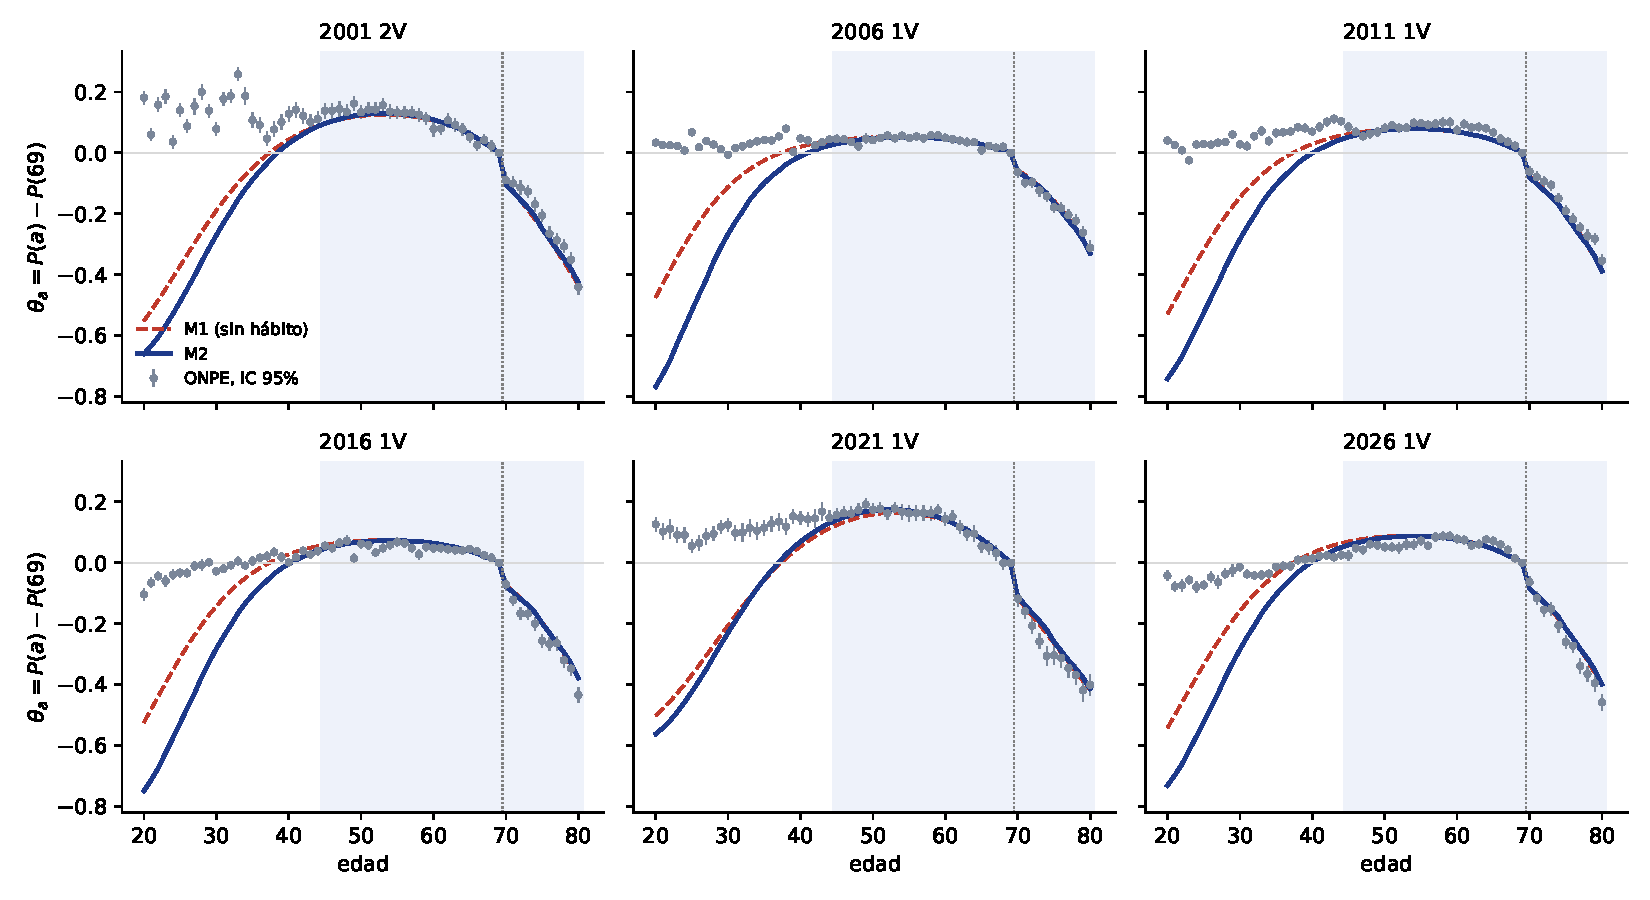
\includegraphics[width=\linewidth]{../code/figures/fit_profiles.pdf}}{}
  \caption{Perfiles $\theta_a=P(a)-P(69)$: datos de la tesis (IC 95\%), modelo sin hábito (M1) y modelo con hábito.
  La zona sombreada es la ventana calibrada. Fuente: \texttt{code/verify.py}.}
  \label{fig:fit}
\end{figure}

La Figura~\ref{fig:fit} muestra el ajuste. Dentro de la ventana el modelo reproduce el perfil
previo a los 70, el salto y la caída posterior. Fuera de ella, entre los 20 y los 45 años, el modelo
proyecta una U invertida que los datos no tienen: la forma $Aa^\alpha-\kappa a^\beta$ no puede ser
plana en la juventud y empinada en la vejez a la vez.

\begin{table}[ht]
  \centering\small
  \caption{Datos frente al modelo, y descomposición de la brecha (Proposición~\ref{prop:bound}).}\label{tab:gap}
  \IfFileExists{../code/output/gap_table.tex}{\resizebox{\linewidth}{!}{\begin{tabular}{lrrrrrrr}
\toprule
 & \multicolumn{2}{c}{$\theta_{70}$} & \multicolumn{2}{c}{$\Delta$} & \multicolumn{3}{c}{Descomposición de $\Delta$ (modelo)} \\
\cmidrule(lr){2-3}\cmidrule(lr){4-5}\cmidrule(lr){6-8}
Elección & datos & modelo & datos & modelo & $\tau^{70}$ & envejec. & hábito \\
\midrule
2001 2V & -0.090 & -0.104 & 0.323 & 0.384 & 0.083 & 0.293 & 0.008 \\
2006 1V & -0.063 & -0.062 & 0.250 & 0.267 & 0.052 & 0.208 & 0.007 \\
2011 1V & -0.062 & -0.081 & 0.313 & 0.342 & 0.067 & 0.266 & 0.009 \\
2016 1V & -0.071 & -0.078 & 0.365 & 0.356 & 0.064 & 0.282 & 0.009 \\
2021 1V & -0.118 & -0.112 & 0.459 & 0.416 & 0.089 & 0.321 & 0.007 \\
2026 1V & -0.064 & -0.086 & 0.393 & 0.374 & 0.071 & 0.295 & 0.009 \\
\bottomrule
\end{tabular}}}{}
  \par\smallskip\footnotesize $\theta_{70}=P(70)-P(69)$. $\Delta$ de los datos: participación de la banda 60--69
  menos la de 70+. La condición (H) se cumple en las seis elecciones calibradas. Fuente: \texttt{code/verify.py}.
\end{table}

\paragraph{¿Cuánto de la brecha es causal?} La Tabla~\ref{tab:gap} contesta la pregunta de la tesis.
En el modelo calibrado el efecto causal de la obligación es $\tau^{70}\in[\tauMin,\tauMax]$, mientras
que la brecha entre grupos en los datos va de \DeltaDataMin{} a \DeltaDataMax{}, y el modelo la
reproduce de cerca. \textbf{Solo entre el \tauShareMin\% y el \tauShareMax\% de la brecha que genera
el modelo calibrado es efecto de la obligación.} El resto es
envejecimiento dentro de una banda abierta que va de los 70 a más de 100 años. El decaimiento del
hábito aporta poco (a lo más \habitDecayMax): con una persistencia tan alta, el hábito se pierde muy
lentamente después de la exención.

\section{Simulaciones}\label{sec:sim}

El script \texttt{code/verify.py} es el único punto de entrada y falla si algún resultado no se
cumple. Comprueba con SymPy la Proposición~\ref{prop:lifecycle} y la estática comparativa del
umbral. Con el modelo de \texttt{code/model.py} verifica las Proposiciones~\ref{prop:jump} a
\ref{prop:rho} sobre sorteos aleatorios de parámetros. La identidad de la
Proposición~\ref{prop:steps} se cumple con un error de $10^{-15}$, porque la grilla del hábito
reparte la masa linealmente y conserva las esperanzas. También recalcula cada objetivo de la
calibración a partir de \texttt{code/data/}, comprueba el anidamiento de M0 a M3 y regenera las
tablas, las figuras y las cifras citadas en el texto.

La comprobación de la Proposición~\ref{prop:bound} encontró un error en su primera formulación,
que pedía solo $a^*\le60$ y un hábito estacionario. En 7 de 150 sorteos con $a^*\le 60$, el hábito
seguía acumulándose entre los 60 y los 70 años y resultaba $\Delta<\tau^{70}$. De ahí la hipótesis
(H), sobre la participación y no sobre $b$. Una simulación sobre sorteos no prueba una proposición:
la verifica en una región de parámetros y puede encontrarle contraejemplos.

\section{Discusión y limitaciones}\label{sec:disc}

\emph{Qué supuesto hace el trabajo.} El resultado central, que la brecha sobrestima el efecto, viene
de la Proposición~\ref{prop:bound} y de su hipótesis (H), que se cumple en la calibración. La
magnitud viene de la pendiente del perfil después de los 70, que la calibración atribuye sobre todo
al ciclo de vida y no al hábito.

\emph{Limitaciones.} (1) El corte transversal mezcla edad y cohorte; los parámetros comunes con un
nivel por elección lo mitigan, pero no lo resuelven. (2) El modelo es estacionario dentro de cada
elección: la historia de cada cohorte se calcula con los parámetros de esa elección. (3) El padrón
incluye fallecidos no depurados, concentrados en los mayores de 70, lo que baja la participación
medida en ese grupo. (4) Hay otras elecciones obligatorias entre presidenciales (regionales,
municipales, referéndums) que también forman hábito y suavizarían los escalones de la
Proposición~\ref{prop:steps}. (5) El ciudadano es miope. (6) La forma de $b$ no ajusta a los jóvenes,
y en el modelo con hábito la persistencia queda en su cota superior.

\section{Conclusión}\label{sec:concl}

\emph{[En preparación.]}

\bibliographystyle{plainnat}
\bibliography{references}

\appendix

\section{Formalización en Lean}\label{app:lean}

\emph{[Pendiente: se corre sobre el commit de este borrador.]}

\section{Registro de colaboración con IA}\label{app:ai}

\emph{[En preparación: ver \texttt{prompts.md}.]}

\end{document}
